\documentclass[dvipdfmx]{jsarticle}

\usepackage[version=3]{mhchem}
\usepackage{amsmath}
\usepackage[siunitx]{circuitikz}
\usepackage{graphicx}
\usepackage{here}

\setlength\parindent{0pt}

\begin{document}
\title{A3実験考察レポート}
\author{03190449  堀 紡希}
\date{\ 8月8日}
\maketitle

\section{考察課題}



\subsection{1.負荷の数と遅延}
実際に実験中にnを1,2,3,4、$V_{DD} = 2.4$V, 周波数1kHzの方形波として測定し、測定した値から最小二乗法により立ち上がり、立ち下がりについてそれぞれ$\tau_{0}, \tau_{1}$が次のように求まった。

  図1が立ち上がりで$\tau_{0} = -7.2$[ns], $\tau_{1} = 17$[ns]


  図2が立ち下がりで$\tau_{0} = 5.1$[ns], $\tau_{1} = 3.9$[ns]

\begin{figure}[H]
\begin{center}
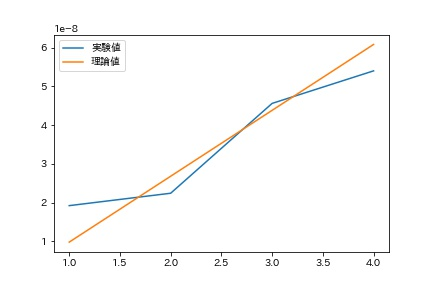
\includegraphics[scale = 0.4]{up.jpg}
\caption{インバータの個数と立ち上がりの遅延とその近侍}
\end{center}
\end{figure}

\begin{figure}[H]
\begin{center}
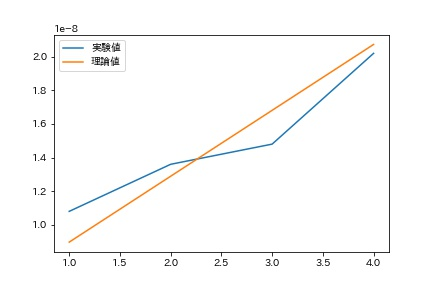
\includegraphics[scale = 0.4]{down.jpg}
\caption{インバータの個数と立ち下がりの遅延とその近似}
\end{center}
\end{figure}

\subsection{2.Dラッチとポジティブ・エッジ・トリガD-FFの動作}
\begin{figure}[h]
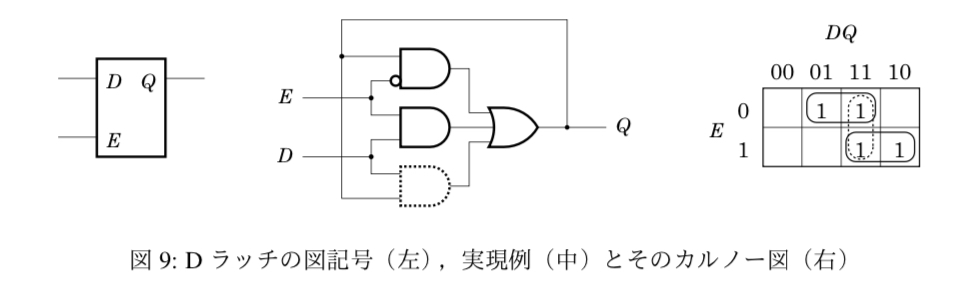
\includegraphics[scale = 0.3]{IMG_0053.jpg}

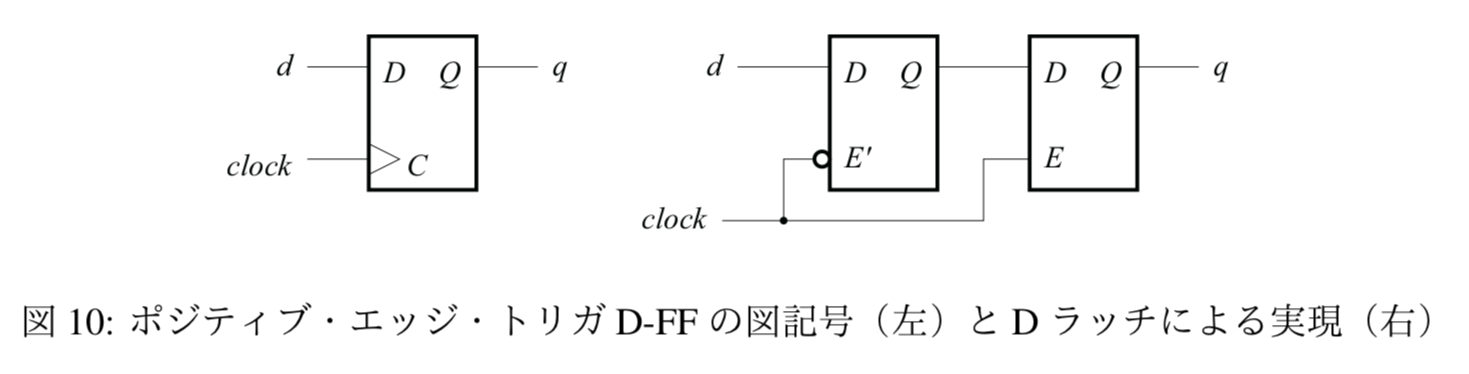
\includegraphics[scale = 0.2]{IMG_0054.jpg}
\end{figure}


これは実験テキストのDラッチとポジティブ・エッジ・トリガD-FFの実現例である。

ゲート一段の遅延を$\tau$とするとDラッチについて、EのANDについているNOTで遅延が発生するのでEがQに到達するまでの遅延はANDゲートが並列になっていることも考えて$3\tau$になる。


ポジティブ・エッジ・トリガD-FFについて、Dラッチが二つ直列になっているので二つ目のDラッチが動作するように$\tau$遅れた二つ目のクロックと一つ目のQが同期すれば良いのでセットアップ時間は$\tau$,ホールド時間はDラッチの遅延時間と同様で$3\tau$。

また、Dラッチの中図で点線で描かれたANDゲートがなくてもカルノー図では確かに正しいが、これがないと$D, Q = (1, 1)$でEが切り替わる時にNOTの遅延により動作が不安定になると考えられるので、それを安定させるためにDQのANDゲートがあると出力がEによらず、安定になると考えられる。



\subsection{3.デジタル回路を部分として構成していく意義}

入力と出力の状態をデジタル化して単純化することにより、定められた入力から出力を返すことさえ守っていれば好きに回路を設計して、組み合わせることが容易であることが、デジタル回路を構成する上での利点である。

また、遅延があまりに大きかったりすると他の部分に影響を及ぼしたりするので、適度なタイミング制約を設定してそれを守ることに留意するべきである。



\section{参考文献}
[1]東京大学工学部:「電気電子情報第一(前期) 実験テキスト」, 2019.

[2]廣瀬明:「電気電子計測」, 数理工学社, 2003.

\end{document}